\documentclass{weekly}
\begin{document}
\maketitlew{Аналитическая механика}{1}{3}{9}

\begin{wrapfigure}[6]{r}{4.5cm}\vspace{-5.5mm}
    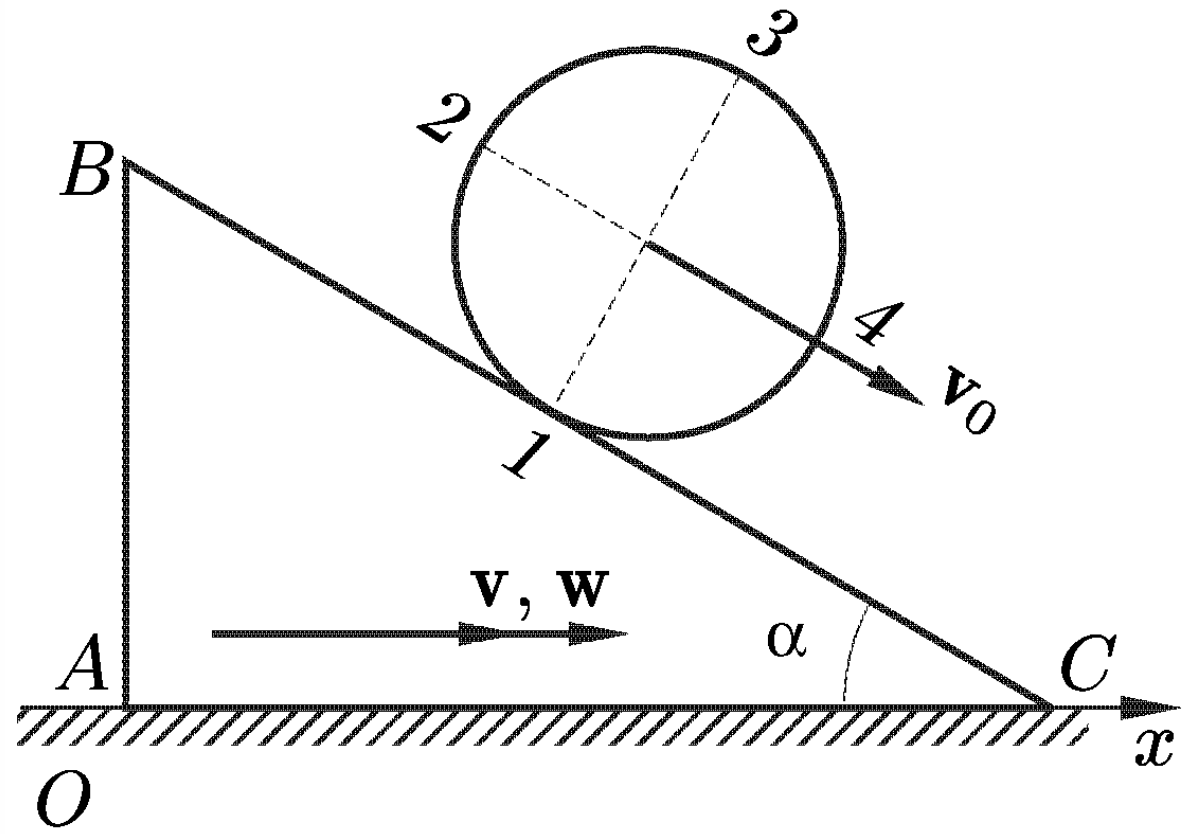
\includegraphics[width=\lw]{2-11}
\end{wrapfigure}
\paragraph{2.11.} Призма~$ABC$ движется поступательно вдоль~оси~$Ox$
с~ускорением~$\vec{w}$, имея в~данный момент скорость~$\vec{v}$.
По~линии наибольшего ската~$BC$ призмы катится без~скольжения
цилиндр, скорость центра которого относительно призмы постоянна
и~равна~$\vec{v_0}$. Радиус цилиндра~$R$, $\angle BCA = \alpha$.
Найти скорости и~ускорения точек~$1, 2, 3, 4$ цилиндра
в~данный момент времени.

$\blacktriangleright$ В~подвижной (штрихованной) системе отсчёта призмы
цилиндр совершает мгновенное вращение вокруг точки~$1$:
$\vec v'_1 = \overline{0}$.
Введём координатные оси: направление~$Ox$ уже задано, $Oy$ направим
вертикально вверх, $\hat z = \hat x \times \hat y$.
\emph{Без~доказательства} заявим, что угловая скорость цилиндра
\begin{equation}
    \vec\omega = -\frac{v_0}{R} \hat z.
\end{equation}

Скорости всех заданных точек найдутся по~формуле Эйлера
($\vec v'_i = \vec\omega \times \vec r_{1i}$):
\begin{align}
    \vec v'_2 &= -\frac{v_0}{R} \hat z \times
            \cvec{\sqrt{2} R\sin\left(\alpha - \frac{\pi}{4}\right)}
            {\sqrt{2} R\cos\left(\alpha - \frac{\pi}{4}\right)}{0}
        = \sqrt{2} v_0
            \left[ \cos\left(\alpha - \frac{\pi}{4}\right) \hat x
            - \sin\left(\alpha - \frac{\pi}{4}\right) \hat y \right]; \\
    \vec v'_3 &= -\frac{v_0}{R} \hat z \times
            \cvec{2R\sin\alpha}{2R\cos\alpha}{0}
        = 2v_0 \left[ \cos\alpha \cdot \hat x -
            \sin\alpha \cdot \hat y \right]; \\
    \vec v'_4 &= -\frac{v_0}{R} \hat z \times
            \cvec{\sqrt{2} R\sin\left(\alpha + \frac{\pi}{4}\right)}
            {\sqrt{2} R\cos\left(\alpha + \frac{\pi}{4}\right)}{0}
        = \sqrt{2} v_0
            \left[ \cos\left(\alpha + \frac{\pi}{4}\right) \hat x
            - \sin\left(\alpha + \frac{\pi}{4}\right) \hat y \right].
\end{align}

Переход к~неподвижной системе отсчёта осуществляется легко и~приятно:
$\vec v_i = \vec v'_i + \vec v$.
\begin{align}
    \vec v_1 &= v \hat x, & \label{2.11:v1}
        v_1 &= v; \\
    \vec v_2 &= \cvec{v + v_0 (\cos\alpha + \sin\alpha)}
            {v_0 (\cos\alpha - \sin\alpha)}{0}, & \label{2.11:v2}
        v_2 &= \sqrt{v^2 + 2v_0^2 +
            2vv_0 (\cos\alpha + \sin\alpha)}; \\
    \vec v_3 &= \cvec{v + 2v_0 \cos\alpha}{-2v_0 \sin\alpha}{0}, &
        \label{2.11:v3}
        v_3 &= \sqrt{v^2 + 4v_0^2 + 4vv_0 \cos\alpha}; \\
    \vec v_4 &= \cvec{v + v_0 (\cos\alpha - \sin\alpha)}
            {-v_0 (\sin\alpha + \cos\alpha)}{0} & \label{2.11:v4}
        v_4 &= \sqrt{v^2 + 2v_0^2 + 2vv_0 (\cos\alpha - \sin\alpha)}.
\end{align}

Ускорение центра цилиндра в~штрихованной системе равно нулю.
Значит, $\vec w'_i = \vec\omega \times \vec\omega \times \vec r_{0i}$:
\begin{align}
    \vec w'_1 &= -\omega^2 R \left[ -\sin\alpha \cdot \hat x -
            \cos\alpha \cdot \hat y \right]; \\
    \vec w'_2 &= -\omega^2 R \left[ -\cos\alpha \cdot \hat x +
            \sin\alpha \cdot \hat y \right]; \\
    \vec w'_3 &= -\omega^2 R \left[ +\sin\alpha \cdot \hat x +
            \cos\alpha \cdot \hat y \right]; \\
    \vec w'_4 &= -\omega^2 R \left[ +\cos\alpha \cdot \hat x -
            \sin\alpha \cdot \hat y \right].
\end{align}
Аналогично, поскольку призма движется поступательно, всё очень приятно:
\begin{align}
    \vec w_1 &= \cvec{w + v_0^2/R \cdot \sin\alpha}
            {v_0^2/R \cdot \cos\alpha}{0}, & \label{2.11:w1}
        w_1 &= \sqrt{w^2 + \frac{v_0^4}{R^2} +
            \frac{2wv_0^2}{R}\sin\alpha}; \\
    \vec w_2 &= \cvec{w + v_0^2/R \cdot \cos\alpha}
            {-v_0^2/R \cdot \cos\alpha}{0}, & \label{2.11:w2}
        w_2 &= \sqrt{w^2 + \frac{v_0^4}{R^2} +
            \frac{2wv_0^2}{R}\cos\alpha}; \\
    \vec w_3 &= \cvec{w - v_0^2/R \cdot \sin\alpha}
            {-v_0^2/R \cdot \cos\alpha}{0}, & \label{2.11:w3}
        w_3 &= \sqrt{w^2 + \frac{v_0^4}{R^2} -
            \frac{2wv_0^2}{R}\sin\alpha}; \\
    \vec w_4 &= \cvec{w - v_0^2/R \cdot \cos\alpha}
            {-v_0^2/R \cdot \sin\alpha}{0}, & \label{2.11:w4}
        w_4 &= \sqrt{w^2 + \frac{v_0^4}{R^2} -
            \frac{2wv_0^2}{R}\cos\alpha}.
\end{align}

\textbf{Ответ:}\quad \eqref{2.11:v1}~-- \eqref{2.11:v4}, ~
\eqref{2.11:w1}~-- \eqref{2.11:w4}.
\hfill $\blacktriangleleft$


\begin{wrapfigure}[6]{r}{4cm}\vspace{-5.5mm}
    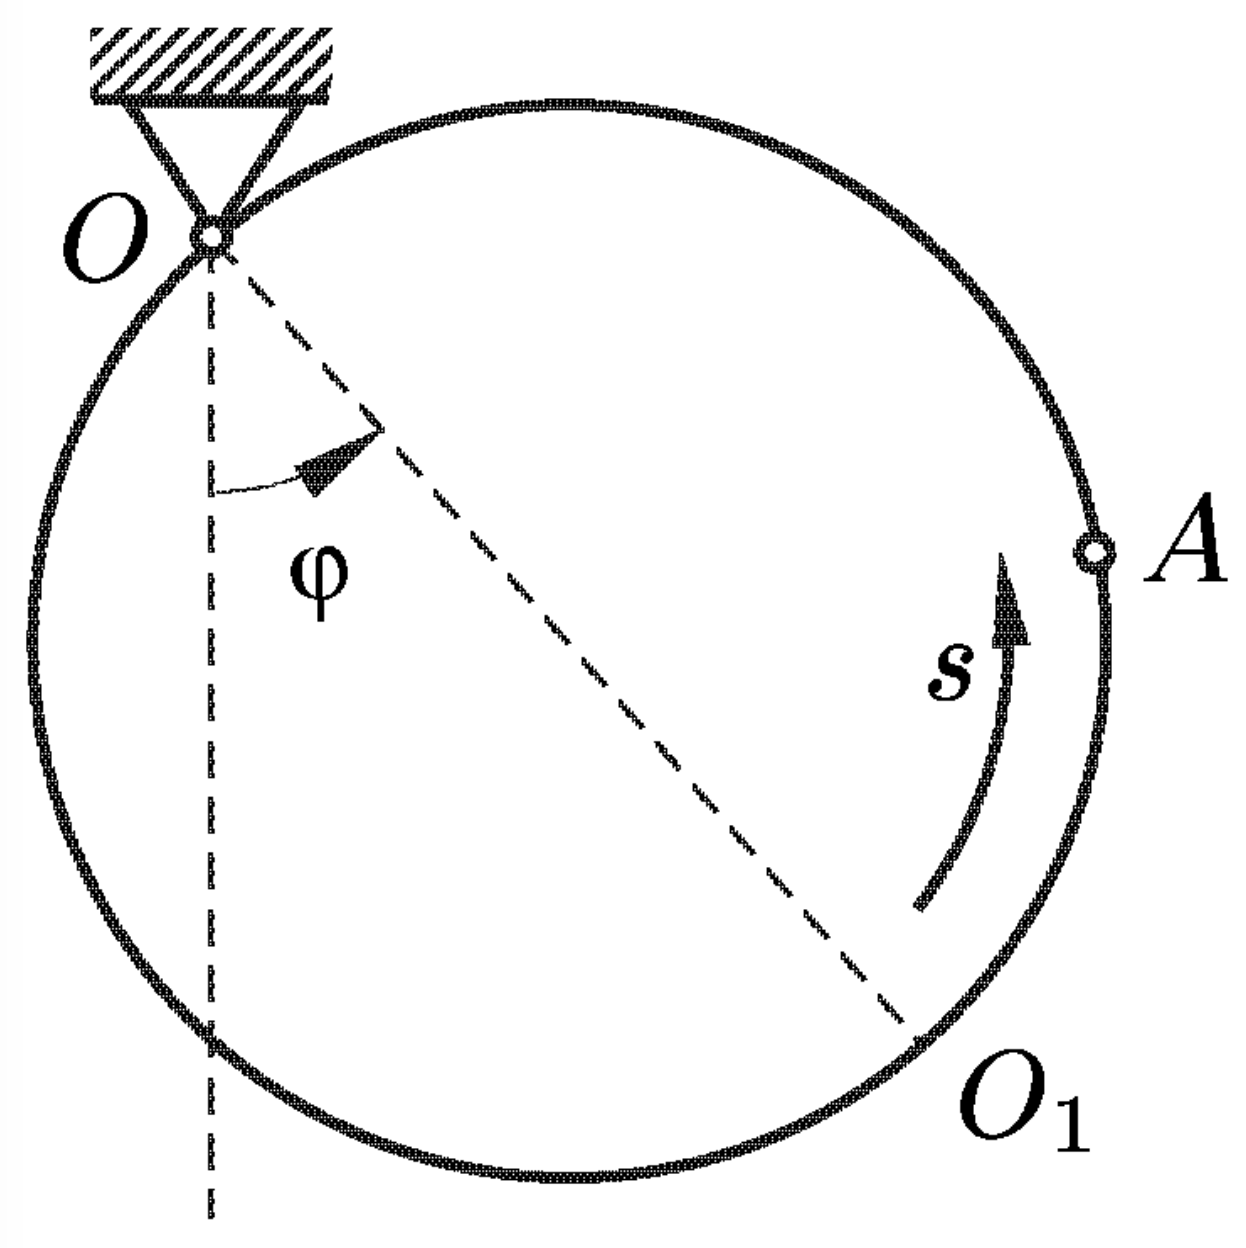
\includegraphics[width=\lw]{2-14}
\end{wrapfigure}
\paragraph{2.14.} Круговое кольцо, точка~$O$ которого неподвижна,
совершает колебания в~своей плоскости по~закону
$\varphi = \varphi_0 \sin\omega t$. Радиус кольца равен~$R$.
Точка~$A$ движется по~кольцу так, что~$s = at^2$, где~$s$~---
длина дуги~$O_1 A$. Найти скорость и~ускорение точки~$A$
в~момент времени~$t = \pi/\omega$.

$\blacktriangleright$ В~заданный момент времени линия~$OO_1$ отвесна.
Введём декартову систему координат: $\hat x \upuparrows OO_1$,
$\hat y$~--- вправо, $\hat z = \hat x \times \hat y$.

В~системе отсчёта кольца
\begin{equation}
\begin{cases}
    x_A = R \left( 1 + \cos\dfrac{s}{R} \right), \\[2mm]
    y_A = R \sin\dfrac{s}{R}.
\end{cases}
\end{equation}
Дифференцируя эти выражения по~времени, получим
компоненты скорости и~ускорения точки~$A$ в~этой системе:
\begin{equation}
\begin{cases}
    \dot x_A = -\sin\dfrac{s}{R} \cdot 2at, \\[4mm]
    \dot y_A = \cos\dfrac{s}{R} \cdot 2at;
\end{cases} \then
\begin{cases}
    \ddot x_A = -\cos\dfrac{s}{R} \cdot \dfrac{4a^2 t^2}{R} -
            \sin\dfrac{s}{R} \cdot 2a, \\[4mm]
    \ddot y_A = -\sin\dfrac{s}{R} \cdot \dfrac{4a^2 t^2}{R} +
            \cos\dfrac{s}{R} \cdot 2a.
\end{cases}
\end{equation}

Угловая скорость и~угловое ускорение кольца
\begin{align}
    \vec\Omega &= -\varphi_0 \omega \hat z; \\
    \vec\varepsilon &= \overline{0}.
\end{align}

Можем теперь применить теоремы о~сложении скоростей и~ускорений:
\begin{align}
\begin{split}
    \vec v_A &= \vec\Omega \times \vec r_A + \vec v'_A = \\
        &= -\varphi_0 \omega R \hat z \times
            \cvec{1 + \cos\frac{at^2}{R}}
            {\sin\frac{at^2}{R}}{0} +
            2at \cvec{-\sin\frac{at^2}{R}}{\cos\frac{at^2}{R}}{0}
        = \cvec{\left[\varphi_0 \omega R -
            \frac{2a\pi}{\omega} \right]\sin\frac{a\pi^2}{\omega^2 R}}
            {-2\varphi_0 \omega R \cos^2\frac{a\pi^2}{2\omega^2 R} +
            \frac{2a\pi}{\omega} \cos\frac{a\pi^2}{\omega^2 R}}{0}.
        \label{2.14:vA}
\end{split}
\end{align}
\textsl{Примечание.} Проверка совпадения модуля~$\vec v_A$
с~ответом из~задачника представляет собой
весьма занимательное занятие. На~сей раз с~этим
помогает справиться~Wolfram Alpha. \emph{Для~$\vec w_A$
аналогичная проверка производиться не~будет.}
\begin{align}
\tag*{}
    \vec w_A &= \vec\varepsilon \times \vec r_A -
            \Omega^2 \vec r_A + \vec w_A' +
            2\vec\Omega \times \vec v_A'
        = - \varphi_0^2 \omega^2
            \cvec{1 + \cos\frac{at^2}{R}}{\sin\frac{at^2}{R}}{0} +
            \cvec{-\frac{4a^2 t^2}{R}\cos\frac{at^2}{R} -
            2a\sin\frac{at^2}{R}}
            {-\frac{4a^2 t^2}{R}\sin\frac{at^2}{R} +
            2a\cos\frac{at^2}{R}}{0} -\\[1ex]&-
            2\varphi_0 \omega \hat z \times
            2at \cvec{-\sin\frac{at^2}{R}}{\cos\frac{at^2}{R}}{0}
        = \cvec
            {-\frac{4a^2 \pi^2}{\omega^2 R}\cos\frac{a\pi^2}
                {\omega^2 R} - 2a\sin\frac{a\pi^2}{\omega^2 R} +
                4\varphi_0\pi\omega a \cos\frac{a\pi^2}{\omega^2 R}}
            {-\frac{4a^2 \pi^2}{\omega^2 R}\sin\frac{a\pi^2}
                {\omega^2 R} + 2a\cos\frac{a\pi^2}{\omega^2 R} +
                4\varphi_0\pi\omega a \sin\frac{a\pi^2}{\omega^2 R}}
            {0}. \label{2.14:wA}
\end{align}

\textbf{Ответ:}\quad \eqref{2.14:vA}, \eqref{2.14:wA}.
\hfill $\blacktriangleleft$


\begin{wrapfigure}[6]{r}{7cm}\vspace{-5.5mm}
    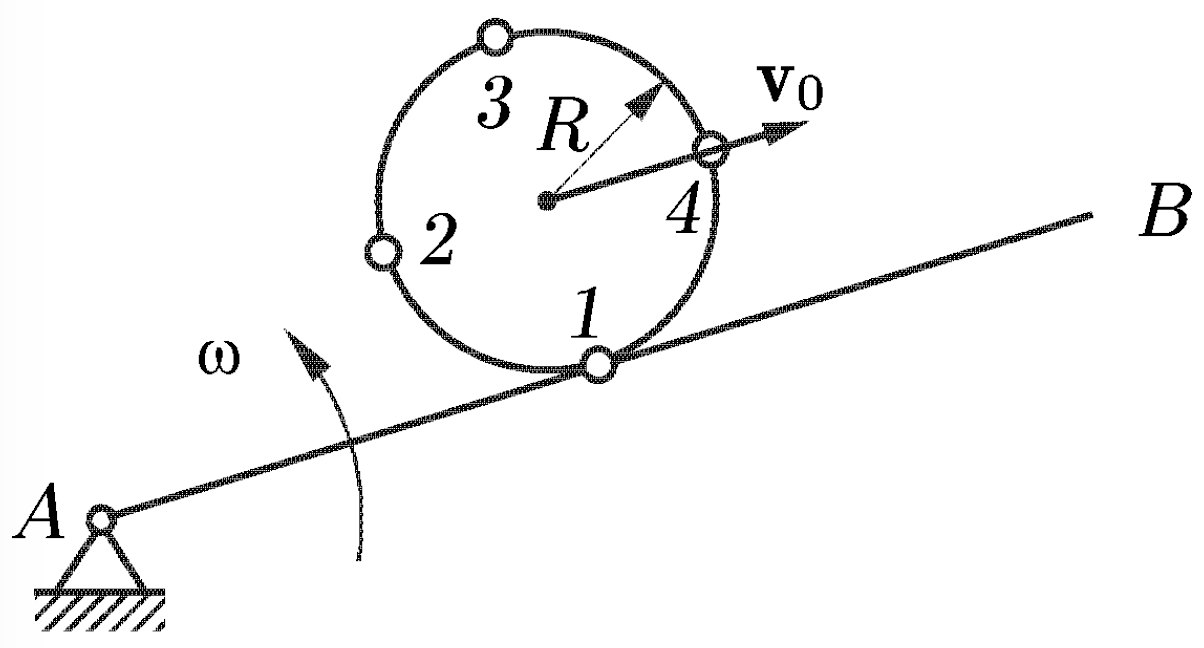
\includegraphics[width=\lw]{3-22}
\end{wrapfigure}
\paragraph{3.22.} Диск радиуса~$R$ катится без~скольжения
по~направляющей~$AB$, вращающейся в~вертикальной плоскости
с~постоянной угловой скоростью~$\omega$. Найти скорости
и~ускорения точек~$1, 2, 3, 4$ диска, если относительная
скорость его центра постоянна и~равна~$v_0$.
В~начальный момент точка касания диска с~направляющей
совпадала с~точкой~$A$.

$\blacktriangleright$ В~подвижной системе отсчёта направляющей
скорости и~ускорения указанных точек
равны соответственно (см.~задачу~2.11)
\begin{align}
    \vec v'_i &= \vec\Omega' \times \vec r_{1i}, \\
    \vec w'_i &= -\Omega'^2 \vec r_{0i};
\end{align}
где~$\Omega' = v_0/R$~--- угловая скорость вращения диска.

Используем теоремы о~сложении скоростей и~ускорений:
\begin{align}
    \vec v_i &= \vec\omega \times \vec r_{Ai} + \vec v'_i
        = \vec\omega \times \vec r_{A1} +
            \left(\vec\omega + \vec\Omega'\right) \times
            \left(\vec r_{0i} - \vec r_{01}\right);
        \label{3.22:vi}
\\
    \vec w_i &= \omega \times \omega \times \vec r_{Ai} + \vec w'_i +
            2\vec\omega \times \vec v'_i
        = \underline{-\omega^2 \vec r_{A1} +
            \left(\omega - 2\Omega'\right)\omega \vec r_{01}} -
            \left(\omega - \Omega'\right)^2 \vec r_{0i}.
        \label{3.22:wi}
\end{align}

Зададимся целью получить ответы в~адекватном виде.
Для этого введём систему координат следующим образом:
$Ax \upuparrows AB$, $Ay \perp AB$ и~направлена вверх,
$\hat z = \hat x \times \hat y$.
В~этой системе все нужные векторы имеют <<красивый>> вид:
\begin{align}
    \vec\omega &= \omega \hat z, \\
    \vec\Omega' &= -\frac{v_0}{R} \hat z; \\[1.5ex]
    \vec r_{A1} &= v_0 t \cdot \hat x;\\
    \vec r_{01} &= -R \hat y, \\
    \vec r_{02} &= -R \hat x, \\
    \vec r_{03} &= +R \hat y, \\
    \vec r_{04} &= +R \hat x.
\end{align}

Осталось произвести вычисления по~формулам~\eqref{3.22:vi}
и~\eqref{3.22:wi}. \hfill $\blacktriangleleft$

\textsl{Например,}
\begin{align}
    \vec v_1 &= \omega v_0 t \cdot \hat z \times \hat x
        = \omega v_0 t \cdot \hat y; \\
    \vec w_1 &= -\omega^2 v_0 t \cdot \hat x -
            \left(\omega - \frac{2v_0}{R}\right)\omega R \cdot \hat y+
            \left(\omega - \frac{v_0}{R}\right)^2 R \cdot \hat y
        = \cvec{-\omega^2 v_0 t}{v_0^2/R}{0}.
\\[2ex]
    \vec v_3 &= \omega v_0 t \cdot \hat z \times \hat x +
            2(\omega R - v_0) \cdot \hat z \times \hat y
        = \cvec{2(v_0 - \omega R)}{\omega v_0 t}{0}; \\
    \vec w_3 &= -\omega^2 v_0 t \cdot \hat x -
            \left(\omega - \frac{2v_0}{R}\right)\omega R \cdot \hat y-
            \left(\omega - \frac{v_0}{R}\right)^2 R \cdot \hat y
        = -\cvec{\omega^2 v_0 t}{2\omega^2 R - 4v_0 \omega +
            \frac{v_0^2}{R}}{0}.
\end{align}


\bigskip
\begin{wrapfigure}[6]{r}{3.3cm}\vspace{-6mm}
    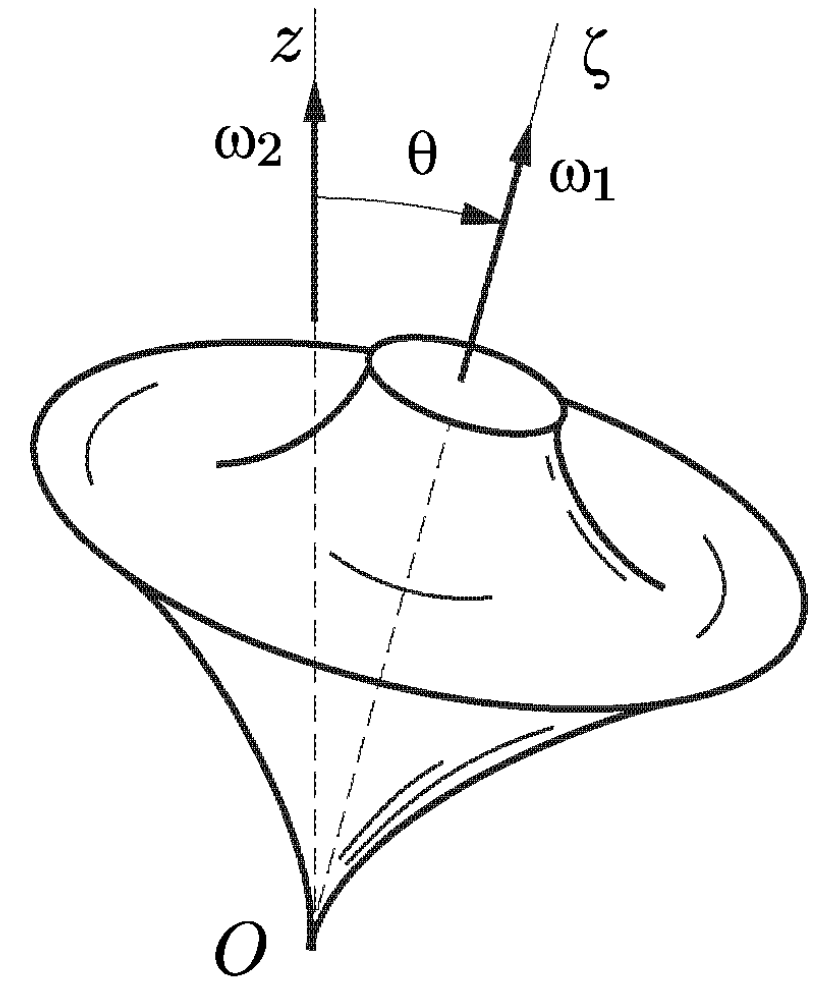
\includegraphics[width=\lw]{4-4}
\end{wrapfigure}
\paragraph{4.4.} Юла вращается вокруг своей оси симметрии~$O\zeta$
с~постоянной угловой скоростью~$\omega_1$. Ось~$O\zeta$
равномерно вращается относительно вертикали~$Oz$ с~угловой
скоростью~$\omega_2$, так~что угол~$\theta$ остаётся постоянным
(регулярная прецессия). Найти угловую скорость и~угловое ускорение
юлы относительно~$Oz$.

$\blacktriangleright$ Результирующее вращение юлы происходит
в~данный момент времени с~угловой скоростью и~угловым ускорением
\begin{align*}
    \vec\omega &= \vec\omega_1 + \vec\omega_2, &
    \omega &= \sqrt{\omega_1^2 + \omega_2^2 + 2\omega_1\omega_2};
\\\tag*{$\blacktriangleleft$}
    \vec\varepsilon &= \omega_1 \times \omega_2, &
    \varepsilon &= \omega_1 \omega_2 \sin\theta.
\end{align*}


\clearpage
\begin{wrapfigure}[7]{r}{5.5cm}\vspace{3mm}
    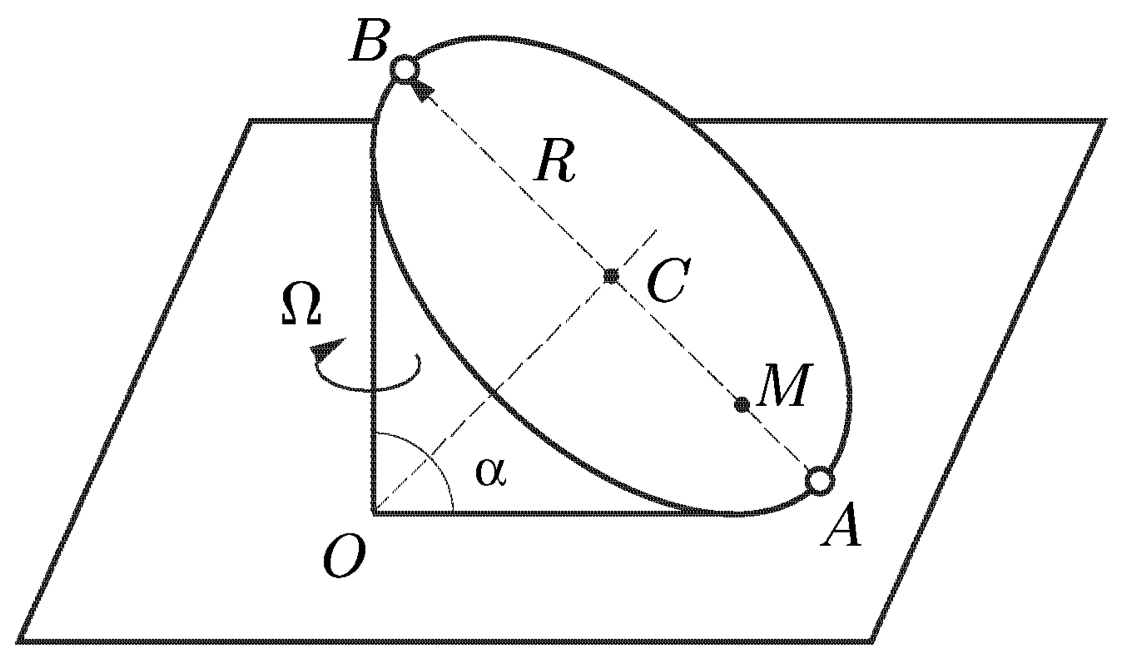
\includegraphics[width=\lw]{4-34}
\end{wrapfigure}
\paragraph{4.34.} Круговой конус с~прямым углом при~вершине
и~радиусом основания, равным~$R$, катится без~скольжения
по~горизонтальной плоскости так, что~скорость центра основания
постоянна и~равна~$v$. Вдоль прямолинейного канала, проведённого
из~вершины~$O$ конуса в~центр~$C$ его основания, равномерно
движется точка со~скоростью, также равной~$v$. Определить
ускорение этой точки в~момент, когда она попадает в~центр основания.

$\blacktriangleright$ Вопрос об~угловых скоростях
в~такой системе \emph{ранее был решён на~семинаре,}
поэтому заявим сразу, что~в~подвижной системе
конус вращается с~угловой скоростью~$\vec\omega'$
вокруг~$OC$, а~сама эта системе~--- c~угловой скоростью~$\Omega$
вокруг~$OB$, так~что конус в~неподвижной системе
совершает мгновенное вращение вокруг~$OA$
с~угловой скоростью~$\omega$:
\begin{equation}
    \vec\omega = \vec\Omega + \vec\omega'.
\end{equation}

Найдём ускорение указанной точки, применив теорему о~сложении
ускорений:
\begin{equation}
    \vec w = \cancel{\vec w'} +
            \vec\Omega\times\vec\Omega\times\overline{OC}
            + 2\vec\Omega \times \vec v'.
\end{equation}
Введём систему координат: $Ox \upuparrows OA$, $Oy \upuparrows OB$,
$\hat z = \hat x \times \hat y$. В~таких координатах
\begin{equation}
    \vec w = \cvec{0}{\Omega}{0} \times \cvec{0}{\Omega}{0} \times
            \cvec{R/\sqrt{2}}{R/\sqrt{2}}{0} +
            2 \cvec{0}{\Omega}{0} \times
            \cvec{v/\sqrt{2}}{v/\sqrt{2}}{0}
        = \cvec{-\Omega^2 R/\sqrt{2}}{0}{-2\Omega v/\sqrt{2}}.
        \label{4.34:w_raw}
\end{equation}

Выразим~$\Omega$ через скорость точки~$C$:
\begin{equation}
    \vec v_C = \Omega \times \overline{OC}
        = \cvec{0}{\Omega}{0} \times
            \cvec{R/\sqrt{2}}{R/\sqrt{2}}{0}
        = \cvec{0}{0}{-\Omega R/\sqrt{2}}
    \then
        v = \frac{\Omega R}{\sqrt{2}}
    \then
        \Omega = \frac{\sqrt{2}v}{R}. \label{4.34:vC}
\end{equation}

Подстановка~\eqref{4.34:vC} в~\eqref{4.34:w_raw} даёт
\begin{align}
    \vec w &= -\cvec{\sqrt{2}}{0}{2} \frac{v^2}{R}; \\
    w &= \frac{\sqrt{6} v^2}{R}.
\end{align}

\textbf{Ответ:}\quad $\vec w = -\cvec{\sqrt{2}}{0}{2} \dfrac{v^2}{R}$.
\hfill $\blacktriangleleft$

\end{document}
